\documentclass[11pt]{article}
\usepackage[ left=2cm, top=3cm, a4paper, text={17cm, 24cm}]{geometry}
\usepackage{graphicx} % Required for inserting images
\usepackage{pdflscape}
\usepackage[T1]{fontenc}
\usepackage{tgschola}
\usepackage[utf8]{inputenc}
\usepackage{hyperref}
\usepackage{float}
\usepackage{xurl}
\usepackage{float}

\title{Návrh projektu/zadania z predmetu ITU}
\author{Jaroslav Mervart, Veronika Kubová, Pavel Hýža, Šimon Dufek}
\date{7 November 2025}

\begin{document}

\begin{titlepage}
\begin{center}
    \Huge
	\textsc{Vysoké učení technické v~Brně}\\
    \huge
	{\textsc{Fakulta informačních technologií }}\\
	
	\vspace{\stretch{0.382}}
	\LARGE
	User Interface Programming\,--\,Final Report\\
	\Huge
    Kimi - \large Digital Pet Webapp\\
	
	\vspace{\stretch{0.618}}
\end{center}
{\large December 14th 2025 \hfill
Veronika Kubová, Šimon Dufek, Pavel Hýža, Jaroslav Mervart}
\end{titlepage}
\newpage

\clearpage
\thispagestyle{empty}
\small
\tableofcontents
\clearpage

\section{Team}

\begin{itemize}
    \item Leader: Jaroslav Mervart
    \item Members: Veronika Kubová, Šimon Dufek, Pavel Hýža
\end{itemize}
Team member Veronika Kubová decided not to work on the project further after the control presentation in week 8 for personal reasons. Her section in this document will not be included.

\section{Kimi - Digital Pet Webapp}
The goal of our project was to design, implement and test a web game application. Users (players) will have to care for a digital pet by tending to its needs and playing mini-games.

Kimi has the following statuses: Hunger, Clean, and Energy. The player has to feed the creature food, clean it using items or the bathroom, and restore its energy with items or the bedroom.

The game has 4 main mini-games: Pinball, Wallball, Brick Breaker, Solitaire. There is also a cooking simulator inside the kitchen room where players can make custom pizzas for Kimi.

The original intention was for there to be a main shop where players would be able to purchase various ingredients for cooking or tending to Kimi's needs in other ways. These items would be purchased through an in-game currency which would be obtainable through playing the various mini-games. However the team member responsible for implementing the main shop and other parts of the application has left the team. Other team members decided to continue focusing on their previously given tasks and parts of the application to demonstrate their respective GUI parts. For this reason there is no real game-mechanic connection between the mini-games and the main game, however the GUI aspects are fully implemented.

The web application is implemented using the Model View Controller scheme. The frontend source files are separated into 3 categories: view, controller, and model. The implementation also contains backend files which are implemented in Python. These files contain API endpoints as well as the implementation of the application's SQLite3 database. The project repository also contains various style CSS source files.

\vspace{1cm}
\textbf{Job distribution:}
\begin{itemize}
    \item Jaroslav Mervart - Main application screen, Achievements, Solitaire mini-game
    
    \item Šimon Dufek - Pizza Kitchen, Inventory, Brick Breaker mini-game
    
    \item Pavel Hýža - Wallball mini-game, Pinball mini-game
\end{itemize}


\newpage

\section{Jaroslav Mervart}

I was responsible for implementing the core frontend infrastructure and several key interactive modules of the application. My work focused on application-wide state management, navigation, shared UI components, and data-driven interaction between the GUI and backend models, following an MVC architecture.

\subsection{Main Application Structure \& Navigation}
\textbf{FE Implementation:}
I co-authored the routing bootstrap in \texttt{frontend/src/main.jsx}, configuring all application routes using \texttt{BrowserRouter}. The main application entry (\texttt{frontend/src/App.jsx}) wires together global Kimi state, controllers, mood handling, inventory access, and navigation entry points.

The architecture ensures that all user interactions (e.g. navigation, actions affecting Kimi) are routed through controllers, which communicate with backend models and trigger UI updates via React state and context.

\subsection{Achievements System}
\textbf{Architecture \& Data Flow:}
I implemented the complete achievements system handling:
\begin{itemize}
    \item Context and provider (\texttt{AchievementContext.jsx}) for global achievement state
    \item Controller for achievement updates (\texttt{achievementController.js})
    \item API-facing model (\texttt{achievementModel.js})
    \item Popup UI component for notifications (\texttt{AchievementInfo.jsx})
\end{itemize}

The achievements menu (\texttt{Achievements.jsx}) consumes the context and dynamically renders unlocked and locked achievements. All achievement state changes originate in the controller, ensuring the GUI never directly manipulates stored data.
\begin{figure}[H]
    \centering
    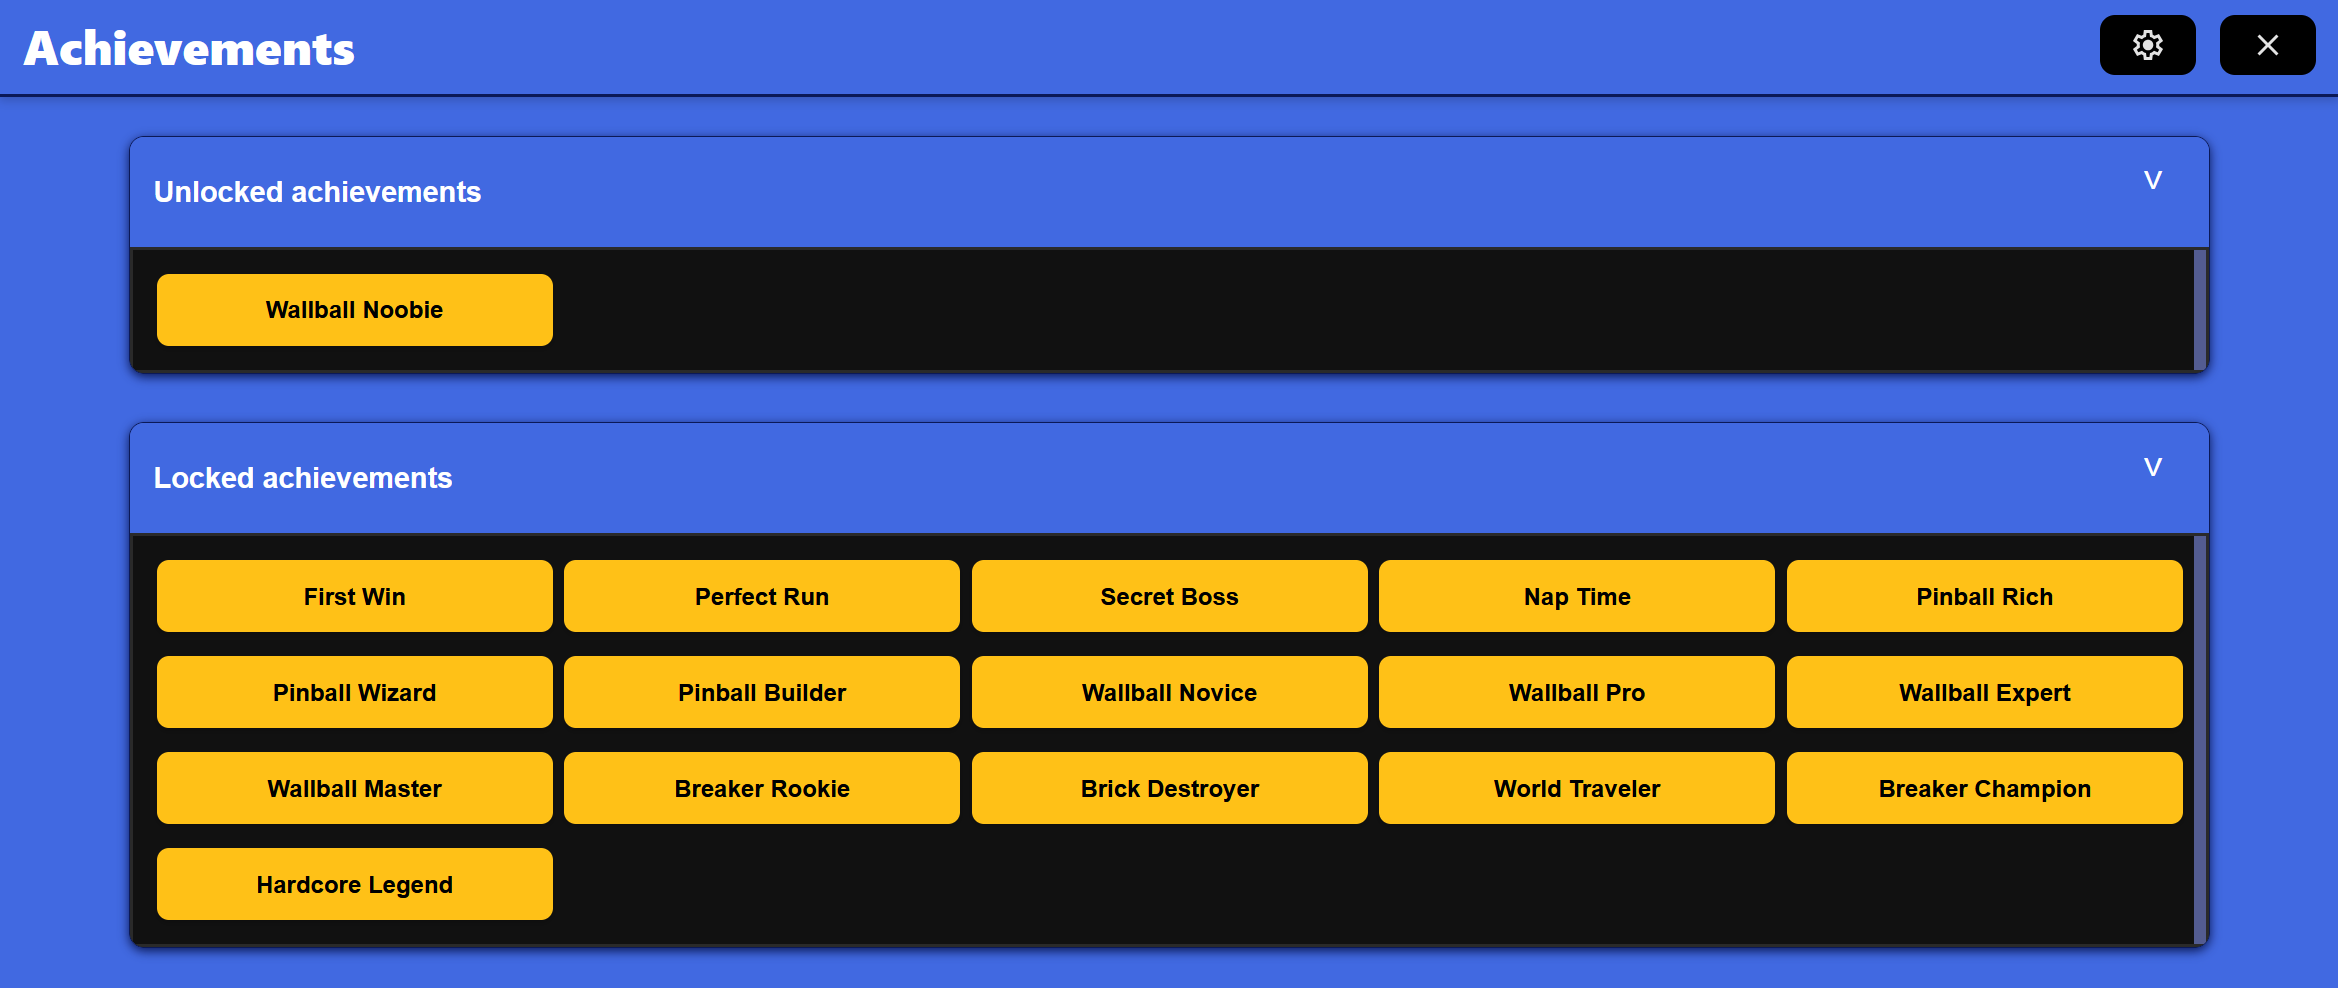
\includegraphics[width=1\linewidth]{pictures/achievements_menu.png}
    \caption{Achievements menu implementation}
    \label{fig:achieve_menu}
\end{figure}

\subsection{Main Scene UI and Kimi Interaction}
\textbf{Shared Interactive Components:}
I developed a set of reusable UI components forming the main scene:
\begin{itemize}
    \item Scene renderer and interactive hotspots (\texttt{Scene.jsx})
    \item Scene object renderer (\texttt{SceneObject.jsx})
    \item Scene carousel for game selection (\texttt{SceneCarousel.jsx})
    \item Header bar (\texttt{Header.jsx})
    \item Kimi status widget (\texttt{KimiStatus.jsx})
    \item Generic status bar component (\texttt{StatusBar.jsx}, co-authored by Veronika Kubová)
\end{itemize}
\begin{figure}[H]
    \centering
    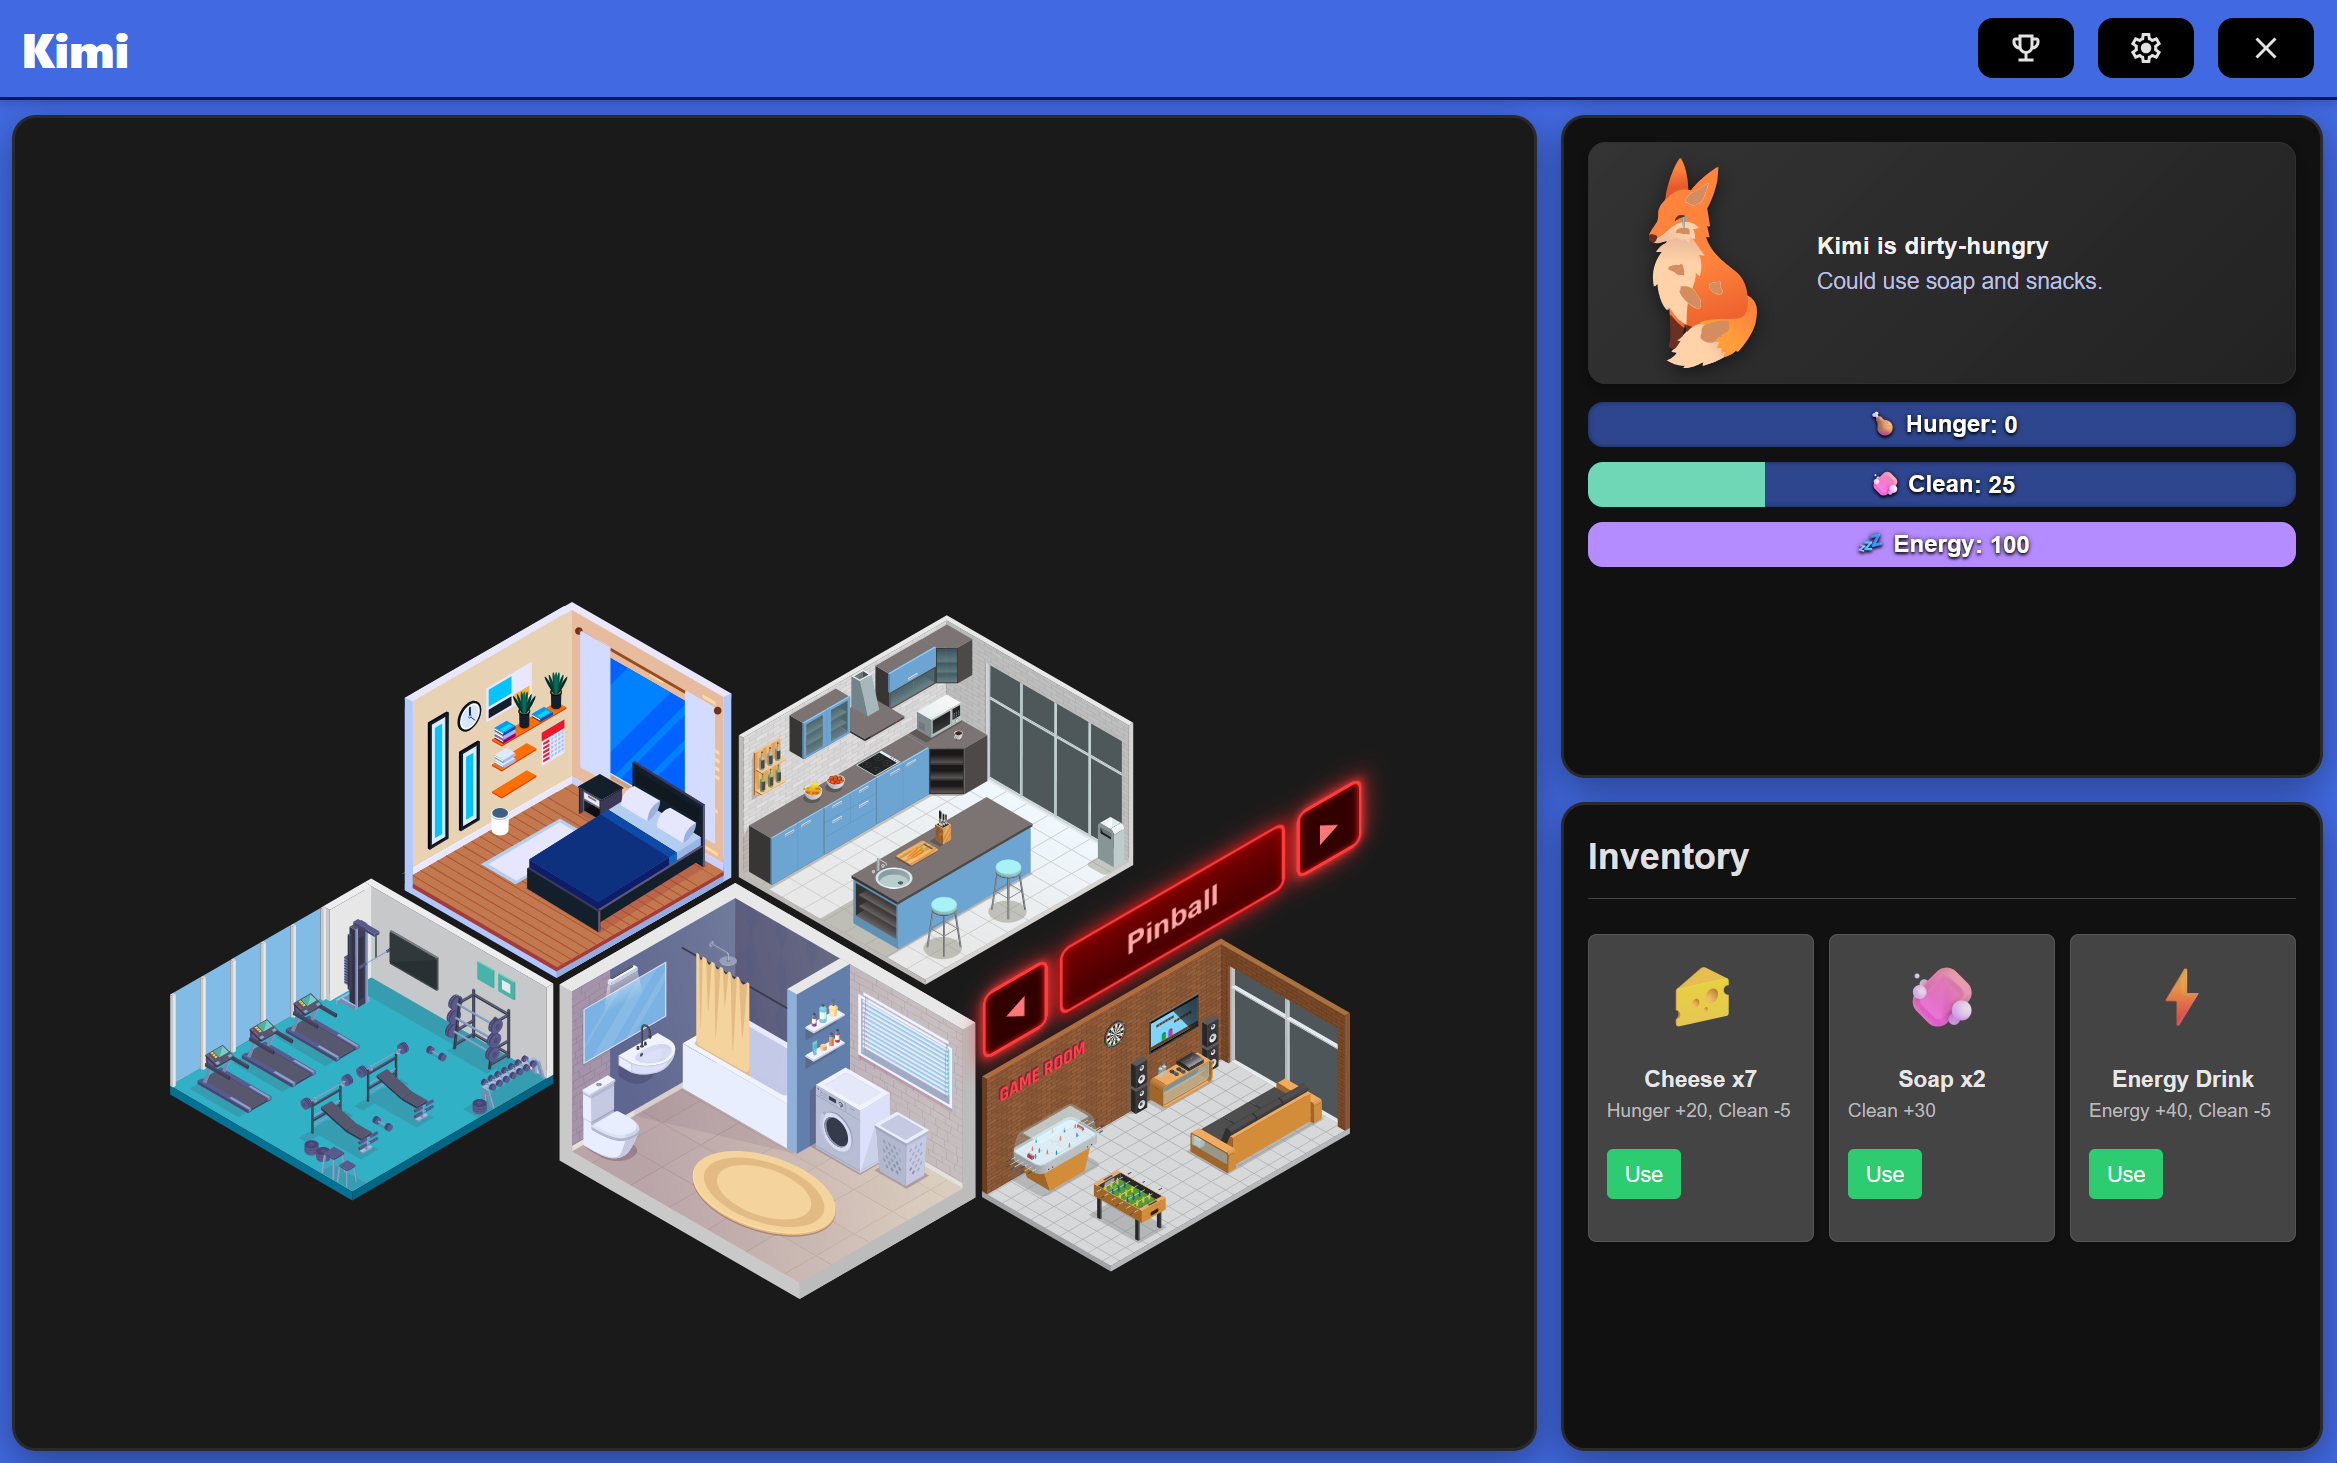
\includegraphics[width=1\linewidth]{pictures/main_menu.png}
    \caption{Achievements menu implementation}
    \label{fig:main_menu}
\end{figure}

Scene layout and interaction data are defined in \texttt{sceneModel.js}. User interactions (clicks on scene objects or carousel actions) are forwarded to controllers, which update Kimi’s state via \texttt{kimiController.js} and \texttt{kimiModel.js}. Updated model values are then reflected back into the UI through React re-rendering.
\newpage
\subsection{Game Module: Klondike Solitaire}
\textbf{FE Implementation:}
I authored the Klondike solitaire view (\texttt{Solitaire.jsx}), implementing:
\begin{itemize}
    \item Full game UI rendering
    \item Win condition detection
    \item Periodic autosave (30s) via timer
    \item Confetti animation upon victory
\end{itemize}
\begin{figure}[H]
    \centering
    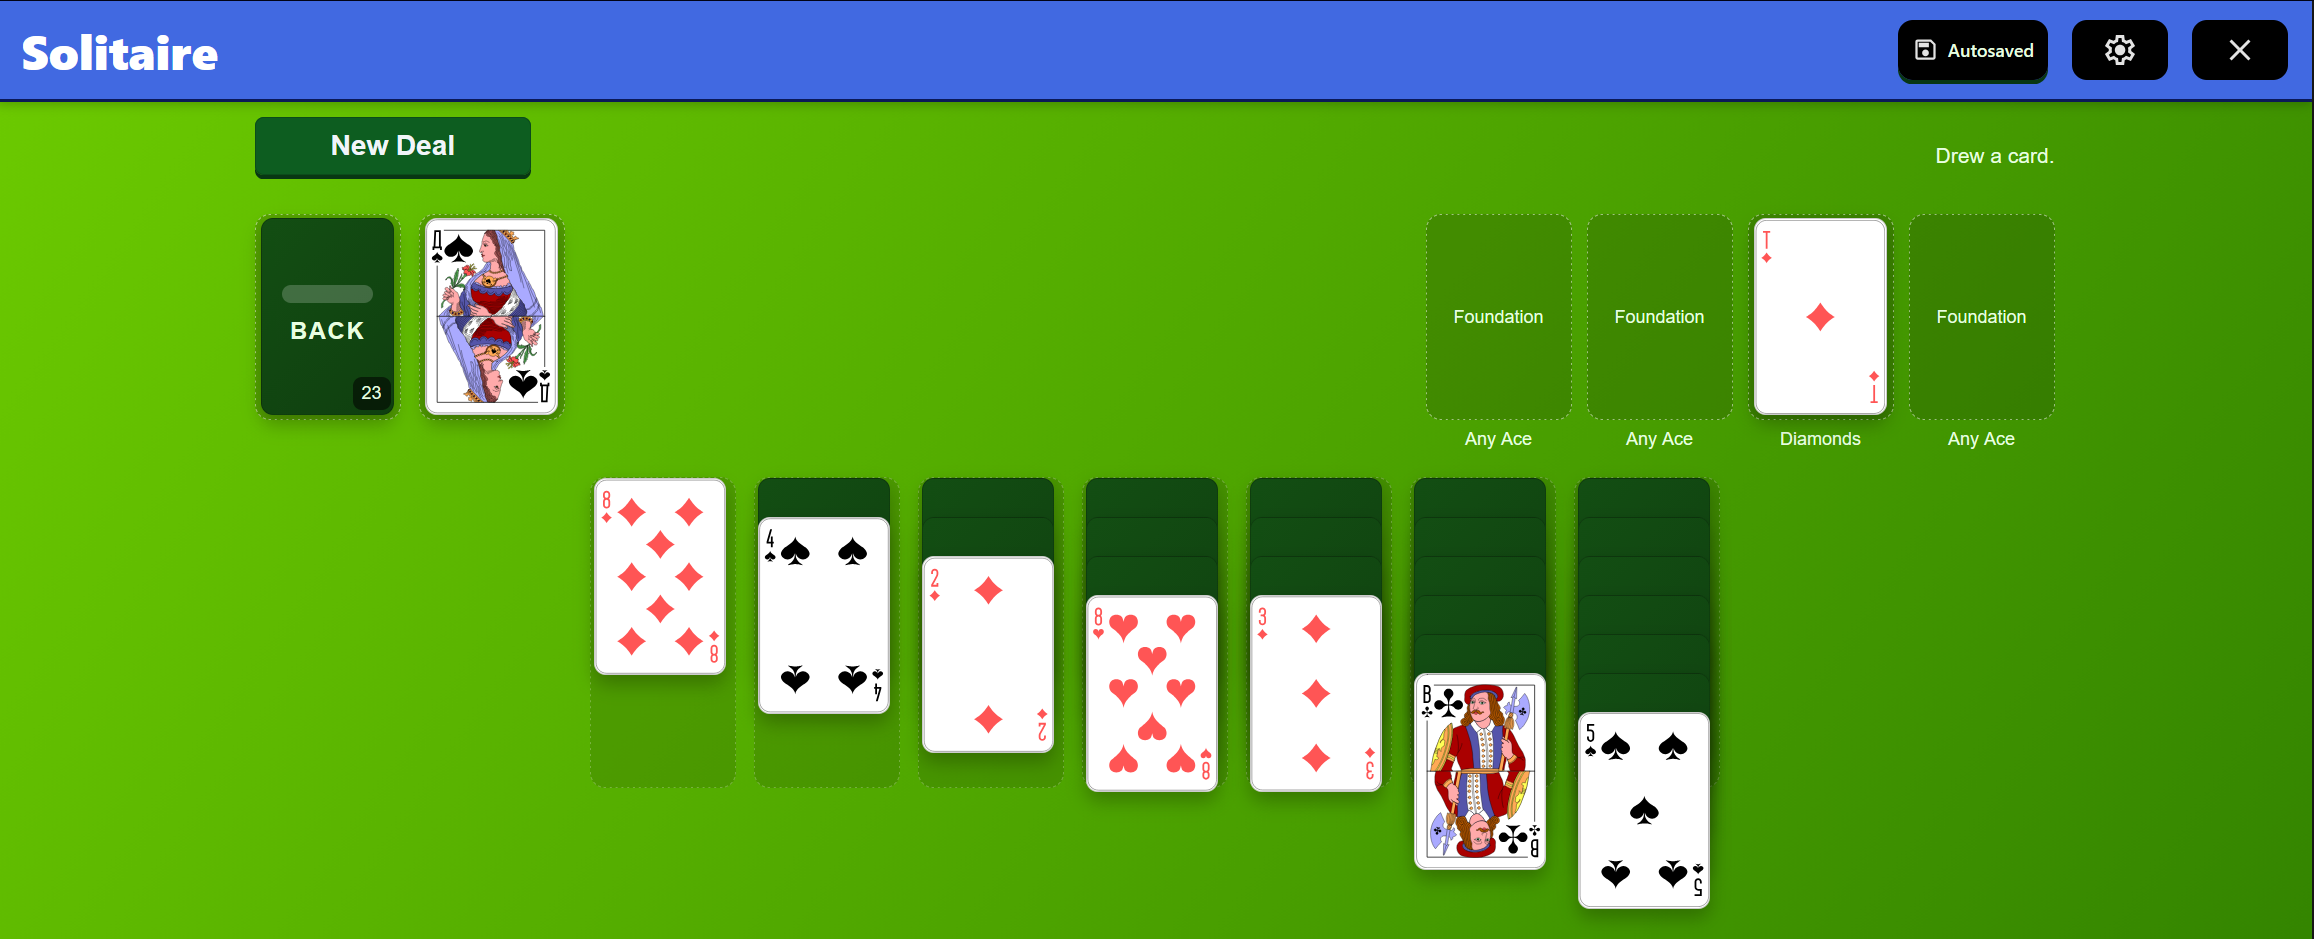
\includegraphics[width=1\linewidth]{pictures/solitaire_menu.png}
    \caption{Solitaire game implementation}
    \label{fig:solitaire_menu}
\end{figure}

Game state changes are managed through a MVC approach, with the UI just rendering the received data. Progress can be saved manually as well, allowing the session to persist. As for the cards themselves, they are not designed by me -- available under public domain \href{https://commons.wikimedia.org/wiki/Category:SVG_complete_decks_of_playing_cards_laid_out#/media/File:Atlasnye_playing_cards_deck.svg}{here}. The cards themselves are contained in a singular \textsc{svg} file, edited in a way where each card has an appropriate id. \textit{SolitaireCard.jsx} uses this file and \textit{solitaireModel.js} to render each card.

\subsection{Settings Menu and Backend Integration}
\textbf{Reset Operations:}
I implemented the settings menu (\texttt{Settings.jsx}) and the corresponding model (\texttt{settingsModel.js}), allowing users to reset achievements, \textit{pinball} records, \textit{breaker} saves, and \textit{wallball} progress. Each action triggers an API call, providing immediate feedback in the UI (e.g. \textsc{Failed to reset pinball record}).
\begin{figure}[H]
    \centering
    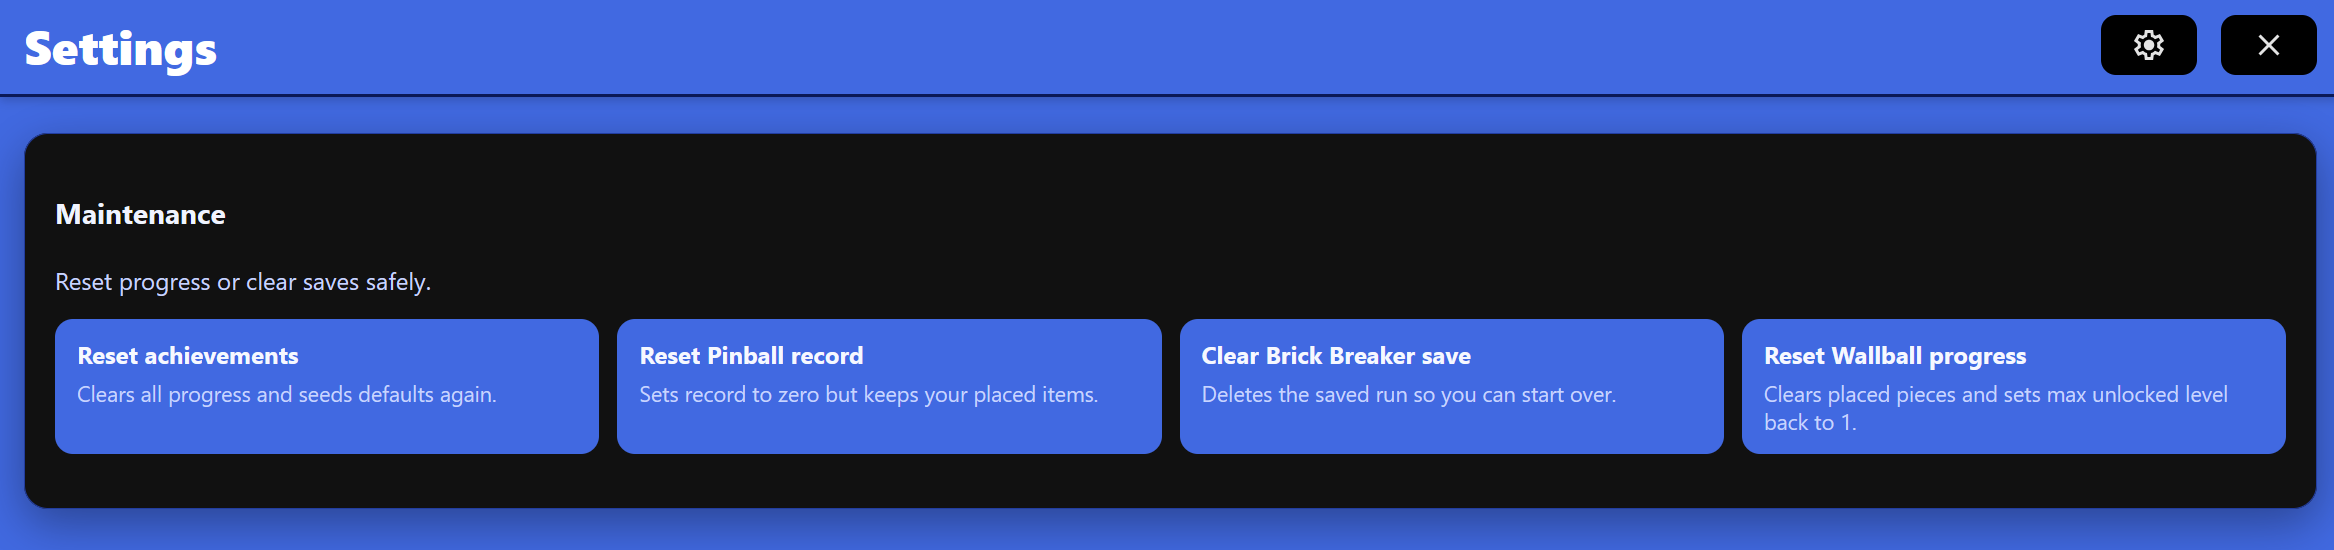
\includegraphics[width=0.85\linewidth]{pictures/setttings_menu.png}
    \caption{Achievements menu implementation}
    \label{fig:settings}
\end{figure}
\subsection{User Testing}
\textbf{Test Participant:}
Testing was conducted with one male participant, 23 years old, identified as an experienced gamer with high technical proficiency.

\begin{itemize}
    \item \textbf{Discoverability and Navigation:}
    The user was observed navigating the application without external guidance. All core interactions were understood within seconds, indicating that scene hotspots and navigation elements were sufficiently intuitive.

    \item \textbf{Visual Feedback:}
    The participant positively reacted to the visual style and clarity of layout. However, they explicitly mentioned that animated transitions or character animations for Kimi would further enhance engagement and perceived responsiveness.

    \item \textbf{Control Comprehension:}
    No moments of hesitation were observed when interacting with scene objects or menus, suggesting that the interaction mapping between UI elements and application actions was clear.
\end{itemize}

\textbf{Key Takeaway:}
While the functional structure and interaction model were validated as intuitive, the testing highlighted animation as a potential area for improvement to strengthen feedback and user engagement.


\newpage
\section{Šimon Dufek}

I was responsible for implementing two complex minigames: the \textit{Pizza Creator} (simulation) and \textit{Brick Breaker} (arcade). Both modules utilize a strict MVC (Model-View-Controller) architecture to separate rendering logic from state management and API communication.

\subsection{Pizza Minigame (Decor \& Baking)}
\begin{figure}[H]
    \centering
    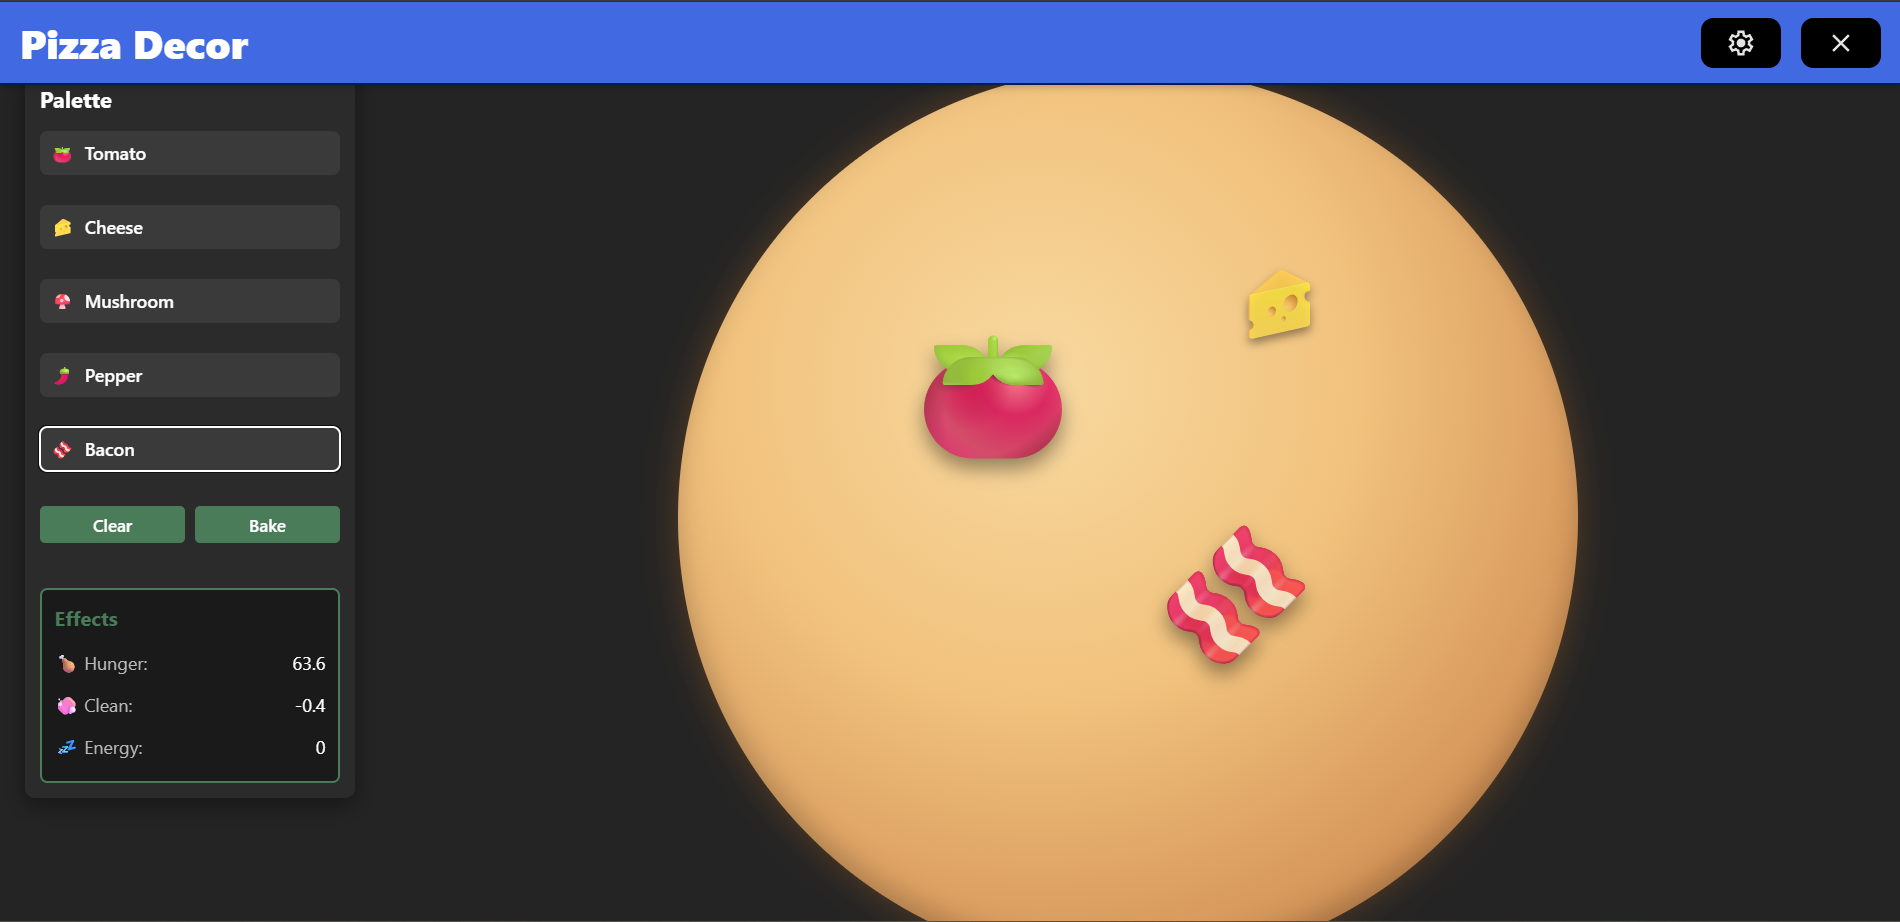
\includegraphics[width=1\linewidth]{pictures/pizza.png}
    \caption{Pizza making Implementation}
    \label{fig:pizza_baker}
\end{figure}
\textbf{FE Implementation:}
The implementation consists of two main views: \texttt{PizzaDecor.jsx} for the drag-and-drop assembly and \texttt{PizzaBaking.jsx} for the simulation of the cooking process. The business logic is encapsulated in \texttt{pizzaController.js} and \texttt{pizzaModel.js}.

\textbf{Interactive Data Manipulation:}
\begin{itemize}
    \item \textbf{Drag and Drop System:} 
    In \texttt{PizzaDecor.jsx}, I implemented a custom pointer-event system. When a topping is dragged, its position is calculated as a percentage relative to the pizza container's dimensions. This ensures the design remains responsive. The \texttt{pointermove} event updates the React state in real-time via the controller, which triggers a re-render of the specific topping component.
    
    \item \textbf{Real-time Stats Calculation:}
    As ingredients are added or removed, the \texttt{PizzaModel} immediately recalculates the nutritional stats (Hunger, Clean, Energy) and checks against defined "Special Recipes". If a recipe match is found, the UI is instantly updated to show the bonus effects.
    
    \item \textbf{Baking Simulation \& API Binding:}
    The baking phase uses a strict internal timer. Upon completion, the \texttt{apiSave} method in the model serializes the entire pizza object (visual composition + calculated effects) and sends it to the \texttt{/pizza/save} endpoint via a POST request. The server then converts this into an inventory item.
\end{itemize}

\textbf{User Testing:}
\textbf{Test Participants:} Validation was performed by 3 individual male users aged 19–26, identified as "Casual Gamers" with a preference for shooter games. Their high technical proficiency and familiarity with game mechanics made them ideal for testing.
\begin{itemize}
    \item \textbf{Interaction Fluidity:} Users tested the custom drag-and-drop implementation on different screen sizes. The feedback confirmed that calculating positions as percentages ($x, y$) effectively maintained the visual layout of toppings regardless of the viewport size.
    \item \textbf{Visual Feedback Clarity:} During the baking phase, users were observed to see if they understood the color-change mechanics. The changing pizza color gradient provided sufficient visual cues for users to stop the timer within the "Perfect" window ($ \pm 1.5s $ from the center) without relying solely on the numerical timer.
    \item \textbf{Recipe Discovery:} Participants successfully identified that specific topping combinations triggered UI updates (the "Matched" badge), confirming that the real-time stat calculation in the model provided immediate and clear feedback.
    \item  \textbf{Minigame Shortcomings:} Users stacked the entire pizza with a huge number of toppings, therefore creating a pizza with a huge nutrition value. This issue was created, because this out application was supposed to have a shop and money mechanics. Each topping was supposed to have a cost, therefore users would be encouraged to not create a pizza with infinite topping. Problems with shops were mentioned in the introduction to our project.
\end{itemize}

\textbf{Source Files:}
\begin{itemize}
    \item \texttt{./frontend/src/PizzaDecor.jsx}
    \item \texttt{./frontend/src/PizzaBaking.jsx}
    \item \texttt{./frontend/src/controllers/pizzaController.js}
    \item \texttt{./frontend/src/models/pizzaModel.js}
\end{itemize}

\subsection{Brick Breaker}
\begin{figure}[H]
    \centering
    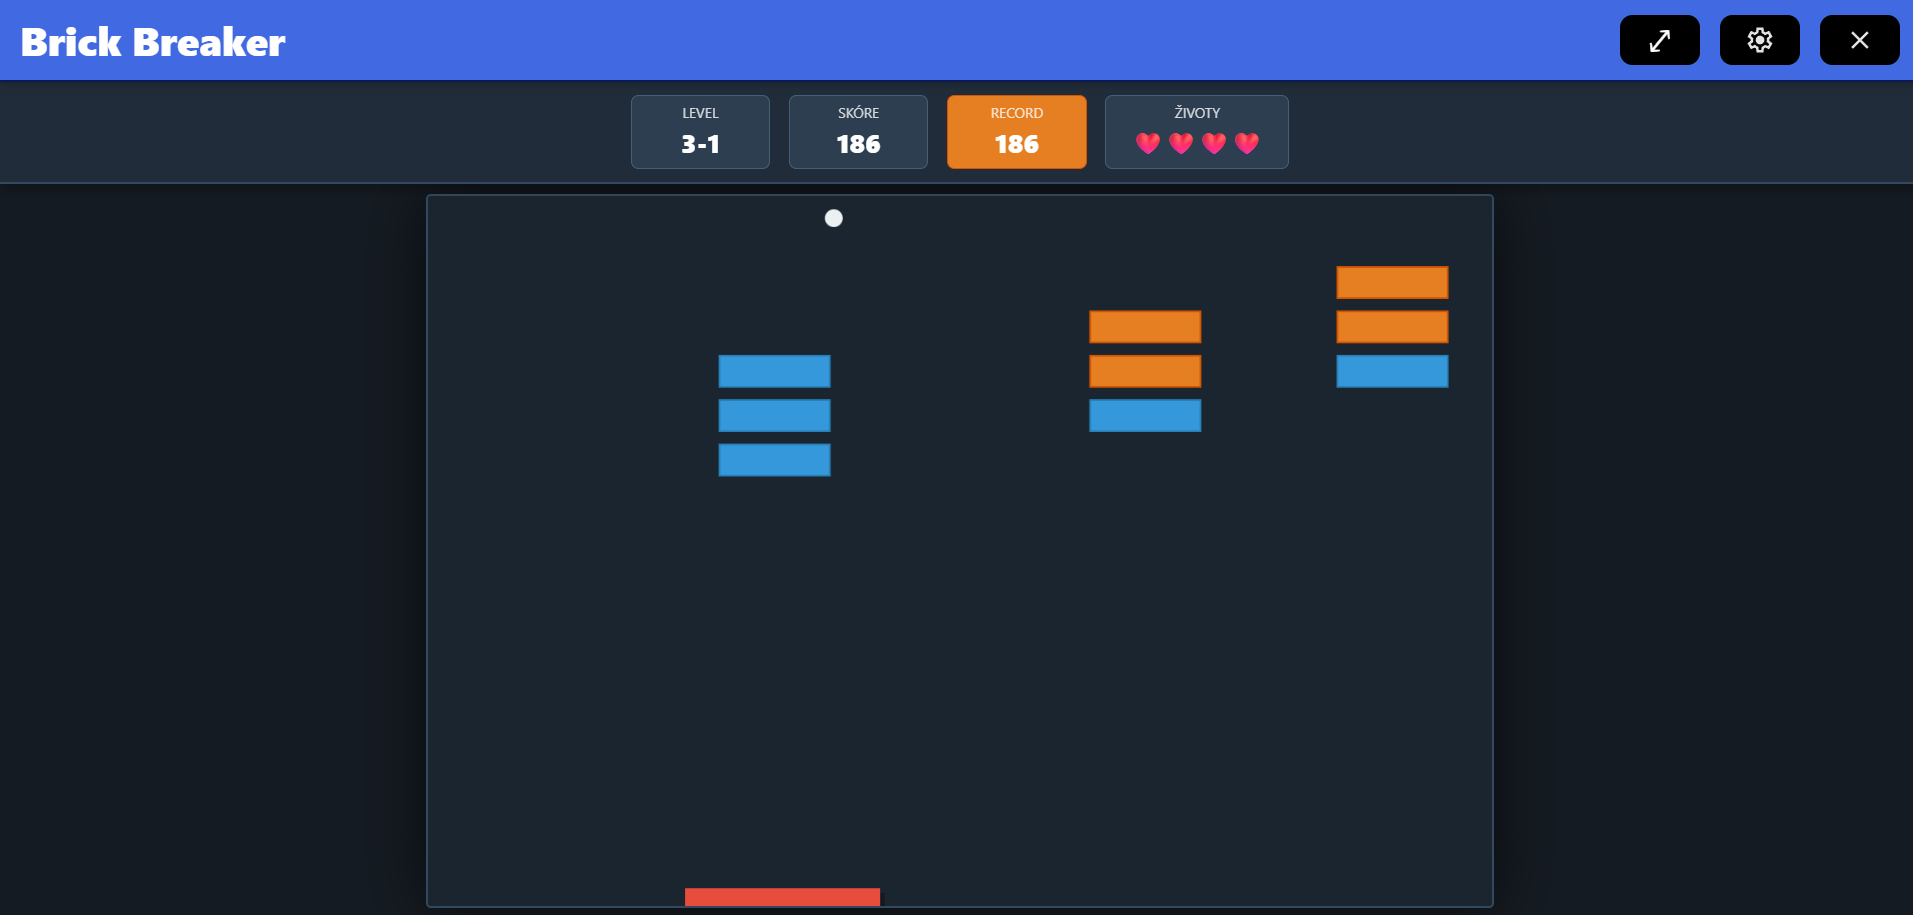
\includegraphics[width=1\linewidth]{pictures/breaker.png}
    \caption{Brick Breaker Implementation}
    \label{fig:brick_breaker}
\end{figure}
\textbf{FE Implementation:}
This is a canvas-based arcade game implemented in \texttt{Breaker.jsx}. Unlike standard React components, the rendering logic here is driven by a high-performance game loop within \texttt{breakerController.js}, which draws directly onto the HTML5 Canvas context.

\textbf{Interactive Data Manipulation:}
\begin{itemize}
    \item \textbf{Physics Engine \& Game Loop:}
    The application state (ball positions, paddle coordinates, brick status) is updated roughly 60 times per second via \texttt{requestAnimationFrame}. The controller handles keyboard inputs to modify the paddle's $x$ coordinate in the state model.
    
    \item \textbf{Automatic State Persistence (Auto-save):}
    To prevent data loss, I implemented an auto-save feature in the controller. The game loop checks the current timestamp against the last save time. If the delta exceeds 1000ms, the entire game state object is serialized and sent to the \texttt{/api/breaker/state} endpoint. This allows the user to refresh the page and resume exactly where they left off.
    
    \item \textbf{Synchronization:}
    Upon component initialization, the controller fetches distinct data sets asynchronously: high scores, unlocked levels, and saved states. These are merged to reconstruct the user's session seamlessly.
\end{itemize}

\textbf{User Testing:}
\textbf{Test Participants:} Validation was performed by 3 individual male users aged 19–26, identified as "Casual Gamers" with a preference for shooter games. Their high technical proficiency and familiarity with game mechanics made them ideal for testing.

Real users played the game in various scenarios to validate controls and data persistence.
\begin{itemize}
    \item \textbf{Input Responsiveness:} Users with different keyboard preferences tested the controls. Based on early feedback, support was added for multiple input schemes (Arrow keys, 'A'/'D', and simple 'Left'/'Right' strings) within the \texttt{handleKeyDown} listener to ensure accessibility for all users.
    \item \textbf{Session Continuity (Auto-save):} Users were instructed to abruptly refresh the browser or navigate away during active gameplay. The testing confirmed that the \texttt{init} function correctly retrieved the serialized state from the server, allowing users to resume exactly where they left off without losing their score or lives.
    \item \textbf{Difficulty Curve:} Users played through the "Normal" and "Hard" difficulties. Feedback indicated that the "Hard" setting's ball speed and narrower paddle width provided a significant challenge, while the visual distinctness of power-ups (e.g., color-coded falling items) was clear and intuitive.
    \item \textbf{Minigame Shortcomings:} Users had a few gripes with my minigame impementation, most of them were aimed at the lack of sound feedback from the minigame and the fact, that the harder difficulties are too hard.
\end{itemize}

\textbf{Source Files:}
\begin{itemize}
    \item \texttt{./frontend/src/Breaker.jsx}
    \item \texttt{./frontend/src/controllers/breakerController.js}
    \item \texttt{./frotend/src/models/breakerModel.js}
    \item \texttt{./frontend/src/breaker\_levels.js}
\end{itemize}

\newpage

\section{Pavel Hýža}

\begin{figure}
    \centering
    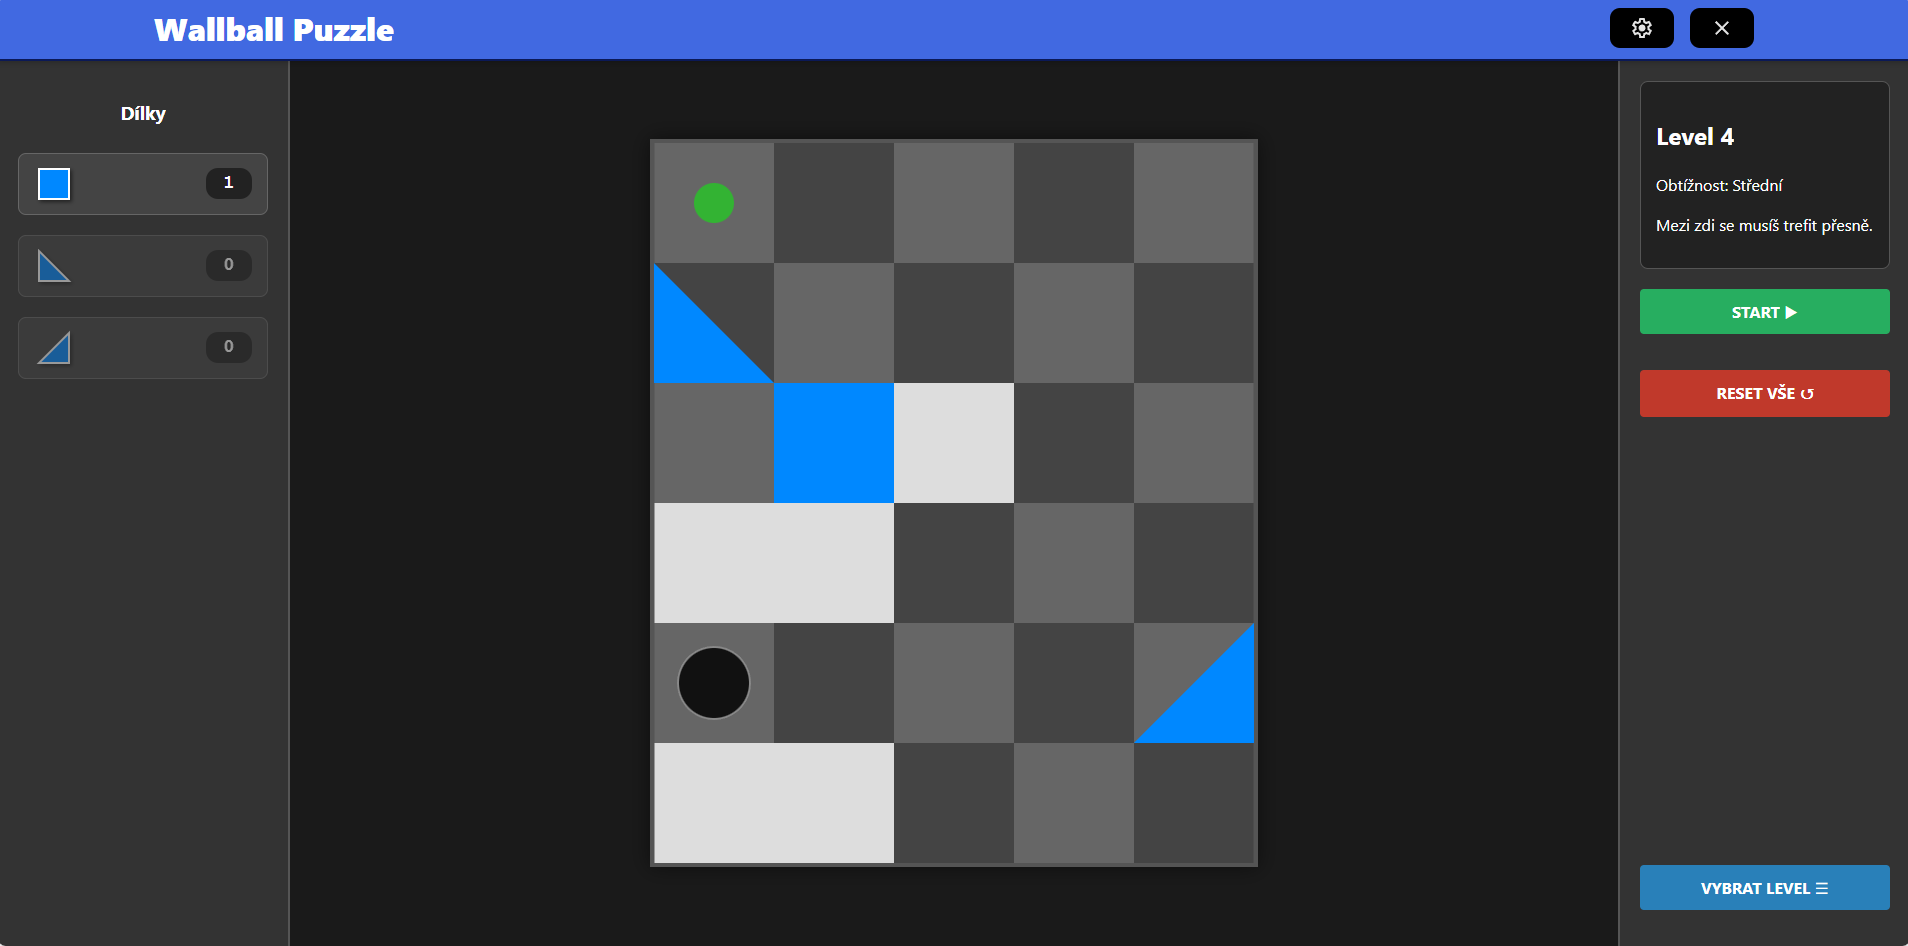
\includegraphics[width=1\linewidth]{pictures/Wallball.png}
    \caption{Wallball Implementation}
    \label{fig:wallball_game}
\end{figure}
\begin{figure}
    \centering
    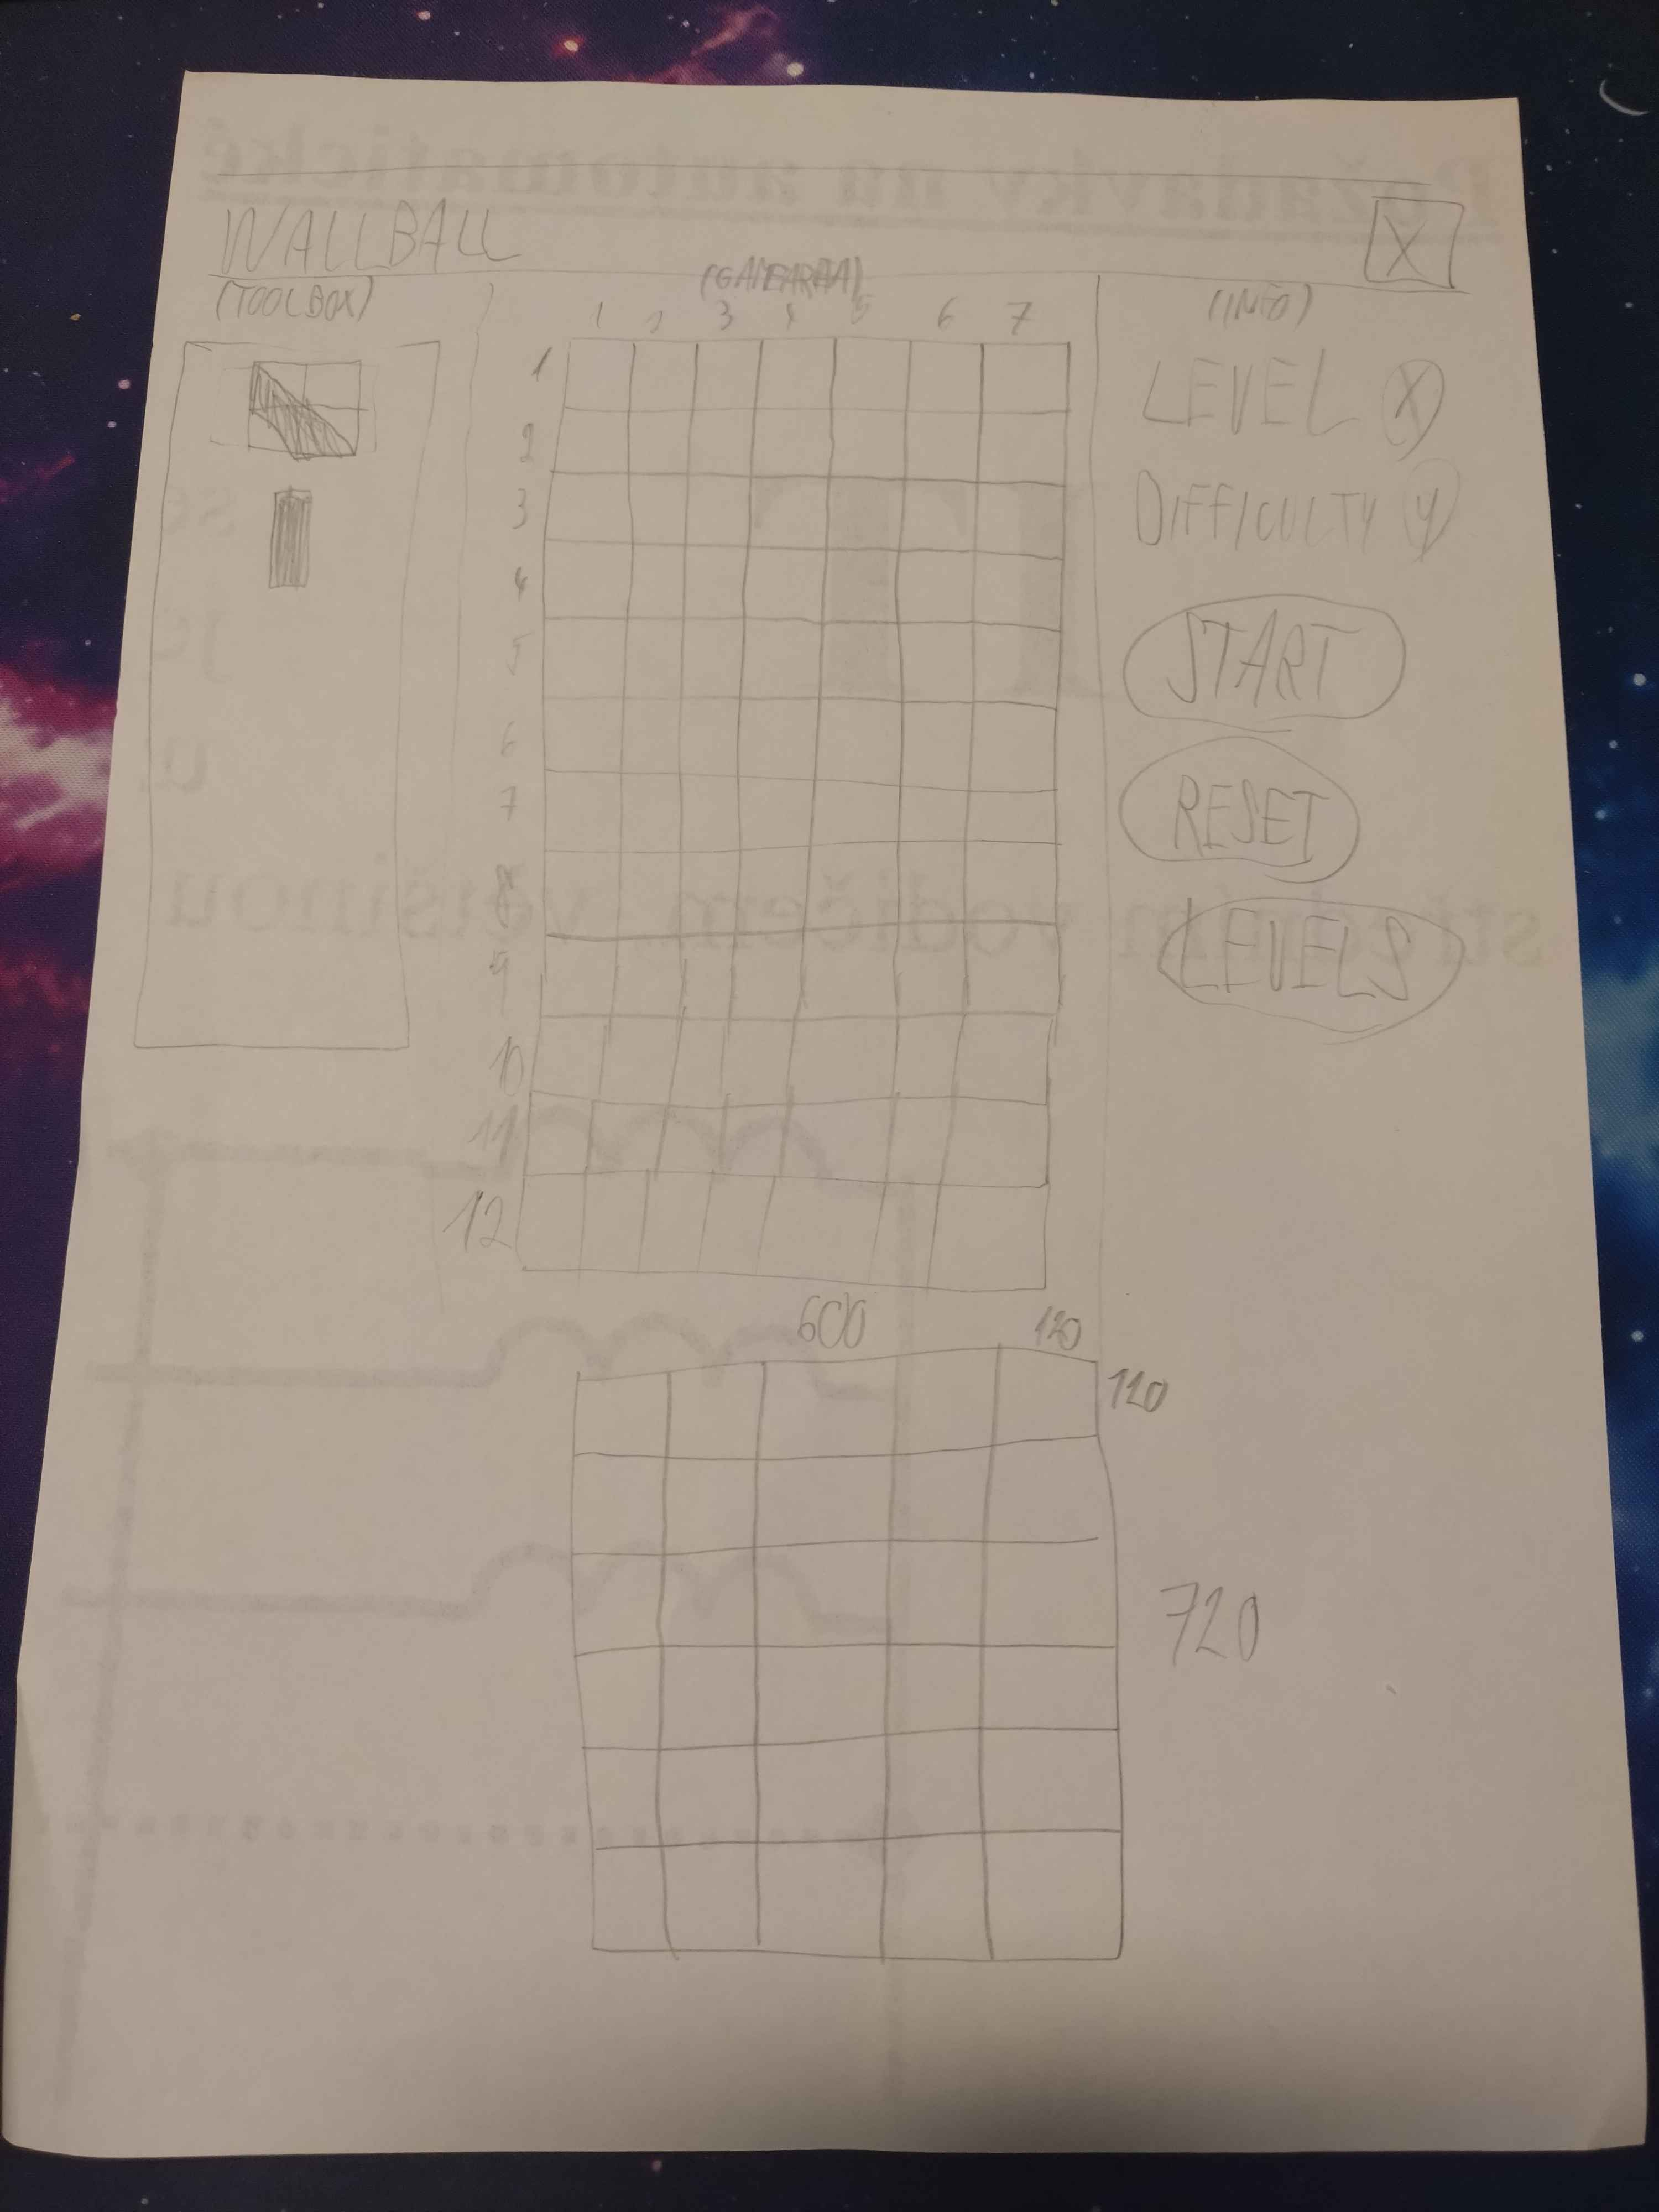
\includegraphics[width=0.9\linewidth]{pictures/Wallball Wireframe.jpg}
    \caption{Wallball Wireframe}
    \label{fig:wallball}
\end{figure}

I was responsible for implementing two physics-based minigames: \textit{Pinball} (arcade builder) and \textit{Wallball} (logic puzzle). Both modules rely on the \texttt{Matter.js} physics engine for rendering and collision detection, employing an MVC architecture to synchronize the frontend state with the backend database.

\subsection{Incorporating feedback from the Control Presentation}
At the control presentation we have received general feedback that there is insufficient "interactive data manipulation", me included. For this reason I decided to move away from the initial idea of having a Dinosaur Runner mini-game. Instead I chose to implement the Wallball logic puzzle game which includes major inline mechanics like drag and drop and better options for "interactive data manipulation". After this mini-game was finished, I completely reworked the Pinball mini-game into the custom builder form, so that it has similar interactivity as Wallball.

\subsection{Wallball (Logic Puzzle)}
\textbf{FE Implementation:}
This game is my unique idea which came to my head as a result of the control presentation and my personal love for sandbox games. The game is implemented in \texttt{Wallball.jsx}. It features a grid-based level design where players must place objects to guide a ball to a goal. The logic is handled by \texttt{wallballController.js}, which manages the transition between the "Edit" mode (placing items) and the "Simulation" mode (physics execution).

\textbf{Interactive Data Manipulation:}
\begin{itemize}
    \item \textbf{Drag and Drop with Visual Feedback:} 
    I implemented a drag-and-drop system allowing users to move geometric shapes from the inventory to the game grid. Based on feedback received shortly before submission, I added a "ghost silhouette" feature. When a user drags an item, a semi-transparent preview of the object follows the cursor, providing immediate visual confirmation of the object's shape and position before placement.
    
    \item \textbf{State Management (Edit vs. Simulate):}
    The controller strictly enforces game states. The inventory is locked while the physics simulation is running. The controller listens for the "Stop" command to reset the ball and unlock the grid for modification.
    
    \item \textbf{Level Persistence:}
    Upon completing a level, the controller communicates with the \path{/api/wallball/complete} endpoint to update the user's progress in the database, unlocking subsequent levels permanently.
\end{itemize}

\textbf{User Testing:}
Testing was conducted with two distinct personas: a "Hardcore Gamer" and a "Non-Gamer" (older generation) to evaluate intuitive design and difficulty curves.
\begin{itemize}
    \item \textbf{Game Flow Understanding:} The non-gamer participant initially struggled with the distinction between the "Play" and "Edit" states. They attempted to drag items while the simulation was running or clicked "Start" before placing any objects. It took approximately two minutes of exploration to understand that the game must be stopped to modify the board. Once this concept was grasped, the user progressed through levels fluidly. It would be worth considering adding a hint mechanic or a more detailed tutorial for less-skilled users.
    \item \textbf{Visual Feedback (Ghost Silhouette):} The gamer participant, while solving all five levels within three minutes, noted a lack of visual precision during dragging. This feedback, corroborated by other team members, led to the implementation of the semi-transparent ghost silhouette mentioned above a few hours before the deadline.
    \item \textbf{Overall Reception:} Both participants liked both mini-games, but both favoured Wallball over Pinball.
\end{itemize}

\textbf{Source Files:}
\begin{itemize}
    \item \texttt{frontend/src/Wallball.jsx}
    \item \texttt{frontend/src/controllers/wallballController.js}
    \item \texttt{frontend/src/models/wallballModel.js}
    \item \texttt{frontend/src/wallball\_levels.js}
\end{itemize}

\subsection{Pinball (Arcade Builder)}
\textbf{FE Implementation:}
Implemented in \texttt{Pinball.jsx}, this game is a reworked version of the Pinball mini-game I presented at the control presentation. Unlike the original, it combines classic arcade gameplay with a sandbox builder. The user can buy extra bumpers and obstacles to customize the table. The physics loop is managed by the controller, which handles the flipper mechanics and collision events.

\textbf{Interactive Data Manipulation:}
\begin{itemize}
    \item \textbf{Shop \& Economy System:}
    The game features an interactive shop. When an item is dragged from the shop to the board, the controller verifies the user's balance. If sufficient funds are available, the item is instantiated in the \texttt{Matter.js} world, the cost is deducted, and the new state is synchronized with the backend via \texttt{/api/pinball/buy}.
    
    \item \textbf{Input Handling:}
    The controller maps keyboard inputs ('A', 'D', 'Space') to physics forces, controlling the left and right flippers and the plunger respectively.
    
    \item \textbf{Contextual Actions:}
    Right-clicking placed items triggers a "Sell" action, removing the physical body from the world and refunding a portion of the currency.
\end{itemize}

\textbf{User Testing:}
\begin{itemize}
    \item \textbf{Controls Accessibility:} The non-gamer participant experienced initial difficulty synchronizing the 'A' and 'D' keys with the ball's movement. However, the learning curve was short, and proficiency was achieved after a few attempts.
    \item \textbf{Shop Discoverability:} The shop UI was initially overlooked by the non-gamer participant, requiring external prompting to notice the purchasing mechanic. However, once discovered, the drag-and-drop purchase flow was considered intuitive.
    \item \textbf{Contextual Help:} The selling mechanic (removing items) was not immediately obvious. The user successfully utilized the feature only after hovering over the item and reading the tooltip ("Right-click to sell"), validating the importance of UI text hints.
    \item \textbf{Interactivity:} The gamer participant praised the freedom to modify the game board, highlighting the interactivity of the builder mode combined with the arcade physics.
\end{itemize}

\textbf{Source Files:}
\begin{itemize}
    \item \texttt{frontend/src/Pinball.jsx}
    \item \texttt{frontend/src/controllers/pinballController.js}
    \item \texttt{frontend/src/models/pinballModel.js}
\end{itemize}

\begin{figure}
    \centering
    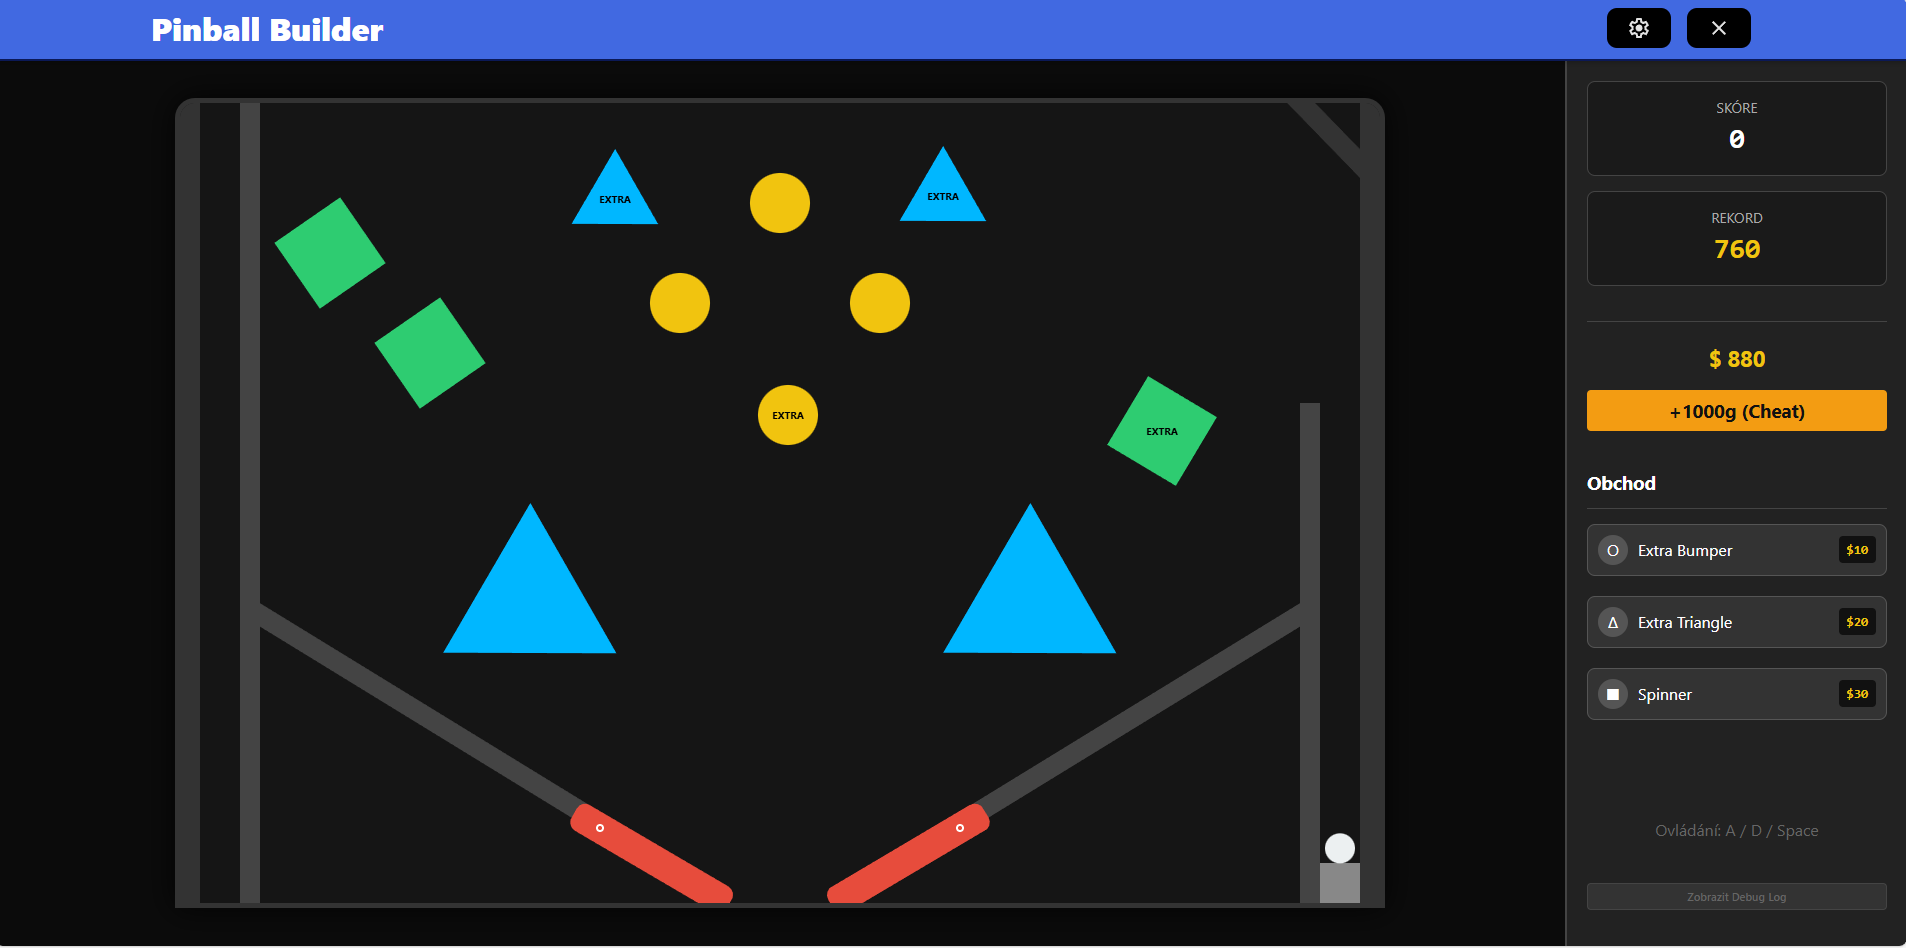
\includegraphics[width=1\linewidth]{pictures/Pinball.png}
    \caption{Pinball Implementation}
    \label{fig:pinball}
\end{figure}

\end{document}